\documentclass[10pt]{article}
\usepackage{amsmath, amssymb, amsthm}
\newcommand{\abs}[1]{\lvert #1 \rvert}
\newtheorem{lemma}{Lemma}
\usepackage[top=2cm, left = 2cm, right = 2cm, bottom = 3cm]{geometry}
\usepackage[pdftex]{graphicx}
\usepackage{asymptote}
\usepackage{tikz}
\usepackage{multicol}
\usepackage{fancyhdr}
\newcommand{\N}{\mathbb{N}}
\pagestyle{fancy}
\rhead{}
\chead{\includegraphics[scale=0.1]{../CMIMC-header-2018.png}}
\lhead{}
\setlength{\headheight}{43pt}
\rfoot{}
\cfoot{}
\lfoot{}
\newcommand{\proposed}[1]
{
\vspace{5pt}
\noindent\textit{Proposed by #1}
}
\newcommand{\solution}
{
\vspace{5pt}
\noindent\textit{Solution.}\qquad
}
\begin{document}

\begin{center}
\huge\textbf{Computer Science Solutions Packet}\normalsize

\vspace{3pt}
\end{center}

\begin{enumerate}

\item Consider the following two vertex-weighted graphs, and denote them as having vertex sets $V=\{v_1,v_2,\ldots,v_6\}$ and $W=\{w_1,w_2,\ldots,w_6\}$, respectively (numbered in the same direction and way). The weights in the second graph are such that for all $1\le i\le 6$, the weight of $w_i$ is the sum of the weights of the neighbors of $v_i$.
Determine the sum of the weights of the original graph.

\begin{center}
\begin{multicols}{2}

\begin{tikzpicture}

  \def \n {6}
  \def \radius {3cm}
  \def \margin {8} % margin in angles, depends on the radius
  
  \foreach \s in {1,...,\n}
  {
    \node[draw, circle, inner sep=0.25cm] (N-\s) at ({360 - 360/\n * (\s - 1) + 90}:\radius) {$v_\s$};
  }

%   \foreach \number in {1,...,\na}{
%     \foreach \numbera in {\number,...,\n}{
%         \path (N-\number) edge[] (N-\numbera)  edge[] (N-\numbera);
%     }
%   }
  \path (N-1) edge[] (N-5) edge[] (N-5);
  \path (N-1) edge[] (N-6) edge[] (N-6);
  \path (N-2) edge[] (N-3) edge[] (N-3);
  \path (N-2) edge[] (N-4) edge[] (N-4);
  \path (N-2) edge[] (N-6) edge[] (N-6);
  \path (N-3) edge[] (N-4) edge[] (N-4);
  \path (N-3) edge[] (N-5) edge[] (N-5);
  \path (N-5) edge[] (N-6) edge[] (N-6);

\end{tikzpicture}

%(v1,v2,v3,v4,v5,v6) = (2, 3, 4, 6, 8, 9)
%w1 = v5+v6 = 8+9 = 17
%w2 = v3+v4+v6 = 4+6+9 = 19
%w3 = v2+v4+v5 = 3+6+8 = 17
%w4 = v2+v3 = 3+4 = 7
%w5 = v1+v3+v6 = 2+4+9 = 15
%w6 = v1+v2+v5 = 2+3+8 = 13
\begin{tikzpicture}
  \def \n {6}
  \def \radius {3cm}
  \def \margin {8} % margin in angles, depends on the radius
  
%   \foreach \s in {1,...,\n}
%   {
%     \node[draw, circle, inner sep=0.25cm] (N-\s) at ({360 - 360/\n * (\s - 1) + 90}:\radius) {$v_\s$};
%   }

  \node[draw, circle, inner sep=0.25cm] (N-1) at ({360 - 360/\n * (1 - 1) + 90}:\radius) {17};
  
  \node[draw, circle, inner sep=0.25cm] (N-2) at ({360 - 360/\n * (2 - 1) + 90}:\radius) {19};
  
  \node[draw, circle, inner sep=0.25cm] (N-3) at ({360 - 360/\n * (3 - 1) + 90}:\radius) {17};
  
  \node[draw, circle, inner sep=0.25cm] (N-4) at ({360 - 360/\n * (4 - 1) + 90}:\radius) {7};
  
  \node[draw, circle, inner sep=0.25cm] (N-5) at ({360 - 360/\n * (5 - 1) + 90}:\radius) {15};
  
  \node[draw, circle, inner sep=0.25cm] (N-6) at ({360 - 360/\n * (6 - 1) + 90}:\radius) {13};

%   \foreach \number in {1,...,\na}{
%     \foreach \numbera in {\number,...,\n}{
%         \path (N-\number) edge[] (N-\numbera)  edge[] (N-\numbera);
%     }
%   }
  \path (N-1) edge[] (N-5) edge[] (N-5);
  \path (N-1) edge[] (N-6) edge[] (N-6);
  \path (N-2) edge[] (N-3) edge[] (N-3);
  \path (N-2) edge[] (N-4) edge[] (N-4);
  \path (N-2) edge[] (N-6) edge[] (N-6);
  \path (N-3) edge[] (N-4) edge[] (N-4);
  \path (N-3) edge[] (N-5) edge[] (N-5);
  \path (N-5) edge[] (N-6) edge[] (N-6);
  
\end{tikzpicture}

\end{multicols}

\end{center}

\proposed{Misha Ivkov}

\solution
This is the system of equations
\begin{align}
    v_5+v_6 &= 17\\
    v_3+v_4+v_6 &= 19\\
    v_2+v_4+v_5 &= 17\\
    v_2+v_3 &= 7\\
    v_1+v_3+v_6 &= 15\\
    v_1+v_2+v_5 &= 13
\end{align}
Adding either (2) and (6) or (3) and (5) gives $\boxed{32}$


\item Consider the natural implementation of computing Fibonacci numbers:

\begin{tabular}{l}
1: \textbf{FUNCTION} $\text{FIB}(n)$: \\
2:$\qquad$ \textbf{IF} $n = 0$ \textbf{OR} $n = 1$ \textbf{RETURN} 1 \\
3:$\qquad$ \textbf{RETURN} $\text{FIB}(n-1) + \text{FIB}(n-2)$
\end{tabular}

When $\text{FIB}(10)$ is evaluated, how many recursive calls to $\text{FIB}$ occur?

\proposed{Patrick Lin}

\solution
Let $f(n)$ be the number of calls to \texttt{fib} during \texttt{fib}(n). Then
\[f(n) = 2 + f(n-1) + f(n-2)\]
with initial conditions $f(0) = 0$ and $f(1) = 0$. We can easily compute the recursion to get $f(10)=\boxed{176}$.


\item You are given the existence of an unsorted sequence $a_1,\ldots, a_5$ of five distinct real numbers.  The Erdos-Szekeres theorem states that there exists a subsequence of length $3$ which is either strictly increasing or strictly decreasing.  You do not have access to the $a_i$, but you do have an oracle which, when given two indexes $1\leq i < j\leq 5$, will tell you whether $a_i < a_j$ or $a_i > a_j$.  What is the minimum number of calls to the oracle needed in order to identify one such requested subsequence?

\proposed{David Altizio}

\solution
We claim the answer is $\fbox{4}$. It is easy to see that three does not work; one can consider all possible sets of calls and for each one construct an ordering of the $a_i$ which prevents determining a desired sequence.  Now we exhibit a sequence of four calls which works.  First call the oracle on (2,3), (3,4), and (2,4).  This allows us to determine a total ordering of the numbers $a_2, a_3, a_4$.  We now case on which one of these is the median.  If it's $a_3$, (2,3,4) works.  Otherwise, WLOG $a_3 < a_2 < a_4$.  Now call (1,2).  Then if $a_1 < a_2$, then (1,2,4) works; if $a_1 > a_2$, then (1,2,3) works.  We are done.

\item Consider the grid of numbers shown below.

\begin{center}
\begin{verbatim}
                                      20 01 96 56 16
                                      37 48 38 64 60
                                      96 97 42 20 98
                                      35 64 96 40 71
                                      50 58 90 16 89
\end{verbatim}
\end{center}

Among all paths that start on the top row, move only left, right, and down, and end on the bottom row, what is the minimum sum of their entries?

\proposed{Cody Johnson}

\solution
Notice that the path traversing down the fourth column has sum $\fbox{196}$, and it is not hard to see that there are no answers which are less than this.

\textbf{Remark. }In general, such a problem can be solved pretty efficiently by a Dynamic Programming algorithm.


\item An \textit{access pattern} $\pi$ is a permutation of $\{1,2,\dots,50\}$ describing the order in which some $n$ memory addresses are accessed. We define the \textit{locality} of $\pi$ to be how much the program jumps around the memory, or numerically, \[\sum_{i=2}^n\left\lvert\pi(i)-\pi(i-1)\right\rvert.\] If $\pi$ is a uniformly randomly chosen access pattern, what's the expected value of its locality?

\proposed{Cody Johnson}

\solution
Let $E$ denote the expected value of $|\pi(i)-\pi(i-1)|$. Then by linearity of expectation and symmetry, our answer is $(n-1)E$. Consider writing the numbers from $1$ to $n$ out. Then there are $n+1$ gaps between them. Since the places that two bars can be placed are independent and selected at random, the expected value of the size of the gap is $\frac{n+1}3$. Then the answer is $\frac{n^2-1}{3}$. Here the desired quantity is $\frac{50^2-1}{3}=\boxed{833}$.


\item We define $\mathcal{W}_{n,p}$ to be the complete weighted undirected random graph with vertex set $\{1,2,\ldots,n\}$: the edge $(i,j)$ will have weight $\min(i,j)$ with probability $p$ and weight $\max(i,j)$ otherwise. Let $\mathcal{L}_{n,p}$ denote the total weight of the minimum spanning tree of $\mathcal{W}_{n,p}$. Find the largest integer less than the expected value of $\mathcal{L}_{2018,1/2}$.

\proposed{Misha Ivkov}

\solution
We prove that
\[\mathbb{E}[\mathcal{L}_{n,1/2}]=2n-3+\dfrac{1}{2^{n-1}}\]
 (where $\mathbb{E}$ denotes expected value) from which the answer follows.\\
Note that $\mathbb{E}[\mathcal L_{2,1/2}] = \frac{3}{2}$, which is true. Assume this statement is true for $n$. We show it follows for $n+1$. To do this, construct the MSP for the first $n$ vertices. Adding an edge to the $n+1$st vertex will preserve the MSP structure, so $\mathbb{E}[\mathcal L_{n+1,1/2}]=\mathbb{E}[\mathcal L_{n,1/2}] + \mathbb{E}[s]$
where $s$ is the weight of the edge to the $n+1$st vertex. This quantity is
\[\mathbb{E}[s]=\dfrac{n+1}{2^n}+\sum_{i=1}^{n}\dfrac{i}{2^i}=2-\dfrac{1}{2^n}\]
Then 
\[\mathbb{E}[\mathcal{L}_{n+1,1/2}]=2n-1+\dfrac{1}{2^n}\]
and we are done, so the answer is $2*2018 - 3 = \boxed{4033}$.

\item I give you a function \textbf{rand} that returns a number chosen uniformly at random from $[0,T]$ for some number $T$ that you don't know. Your task is to approximate $T$. You do this by calling \textbf{rand} $100$ times, recording the results as $X_1,X_2,...,X_{100}$, and guessing \[\hat{T}=\alpha\cdot\max\{X_1,X_2,...,X_{100}\}\] for some $\alpha$. Which value of $\alpha$ ensures that $\mathbb{E}[\hat{T}]=T$?

\proposed{Cody Johnson}

\solution
Let�s calculate $\mathbb{E}[\hat{T}]$ when $\alpha=1$. We have 
\begin{align*}
\mathbb{E}[\hat{T}] &=\int_0^T\Pr[\hat{T} > x]\,\mathrm dx\\
&=\int_0^T(1-\Pr[\hat{T}\le x])\,\mathrm dx\\
&=\int_0^T(1-\Pr[X_1\le x\land X_2\le x\land...\land X_{100}\le x])\,\mathrm dx\\
&=\int_0^T(1-(x/T)^{100})\,\mathrm dx\\
&=\frac{100}{101}T
\end{align*}
Therefore, the answer is $\alpha=\boxed{\frac{101}{100}}$.


\item We consider a simple model for balanced parenthesis checking. Let $\mathcal R=\{\texttt{(())}\rightarrow \texttt{A},\texttt{(A)}\rightarrow\texttt{A},\texttt{AA}\rightarrow\texttt{A}\}$ be a set of rules for phrase reduction. Then the phrase is balanced if and only if the model is able to reduce the phrase to \texttt{A} by some arbitrary sequence of rule applications. For example, to show \texttt{((()))} is balanced we can do:
\[\texttt{((()))}\rightarrow\texttt{(A)}\rightarrow\texttt{A}\qquad \checkmark\]
Unfortunately, the above set of rules $\mathcal R$ is not complete; find the number of balanced parenthetical phrases of length $14$ for which $\mathcal R$ \textbf{is insufficient} to show that they are balanced.

\proposed{Misha Ivkov and Patrick Lin}

\solution
Let $f(n)$ be the number of phrases which can be shown to be balanced if the length is $2n$, with $f(1) = 0$ and let $g(n) = f(n)$, except $g(1) = 1$. Then we claim
\[f(n) = f(n-1) + \sum_{i=1}^{n-2}g(i)f(n-1-i)\]
This can be shown term by term. $f(n-1)$ represents taking all phrases of length $2n-2$ and adding a set of parens around them. For all the other terms, consider a phrase of length $2n$ as the combination of $(2k)\circ 2(n-k-1)$, with the first parentheses showing that it is indeed attainable. This is why $g(1)=1$ is required, so that the first term exists. The number of ways to create $(2k)\circ 2(n-k-1)$ is $g(k)f(n-k-1)$, as suggested by the formula. Hence we can compute $f(7) = 37$, and the total number of balanced parenthetical phrases of length $14$ is $\frac 18\binom{14}7$ so the answer is $\frac 18\binom {14}7 - 37 = \boxed{392}$.


\item Consider the following modified algorithm for binary search, which we will call \textit{weighted binary search}:

\begin{tabular}{l}
01: \textbf{FUNCTION} SEARCH($L$, value) \\
02:$\qquad$  hi $\leftarrow$ len(L) - 1 \\
03:$\qquad$  lo $\leftarrow$ 0 \\
04:$\qquad$  \textbf{WHILE} hi $\geq$ lo \\
05:$\qquad\qquad$ guess $\leftarrow$ $\lfloor w \cdot\text{lo} + (1-w) \cdot \text{hi}\rfloor$ \\
06:$\qquad\qquad$ mid $\leftarrow$ $L[\text{guess}]$ \\
07:$\qquad\qquad$ \textbf{IF} mid $> \text{value}$ \\
08: $\qquad\qquad\qquad$ hi $\leftarrow$ guess - 1 \\
09: $\qquad\qquad$ \textbf{ELSE IF} mid $< \text{value}$ \\
10: $\qquad\qquad\qquad$ lo $\leftarrow$ guess + 1 \\
11: $\qquad\qquad$ \textbf{ELSE} \\
12: $\qquad\qquad\qquad$ \textbf{RETURN} guess \\
13:$\qquad$ \textbf{RETURN} -1 (not found) 
\end{tabular}\\

Assume $L$ is a list of the integers $\{1,2,\ldots,100\}$, in that order. Further assume that accessing the $k$th index of $L$ costs $k+1$ tokens (e.g. $L[0]$ costs $1$ token). Let $S$ be the set of all $w\in[0.5,1)$ which minimize the average cost when \texttt{value} is an integer selected at random in the range $[1,50]$. Given that $S=\left(x,\frac {74}{99}\right]$, determine $x$.

\proposed{Misha Ivkov}

\solution
Notice that all optimal values will have the property that $\lfloor wa+(1-w)b \rfloor = \lfloor \frac{74a+25b}{99}\rfloor$. This can be rewritten as
\[\lfloor w(a-b) \rfloor = \left\lfloor \frac{74}{99}(a-b)\right\rfloor\]
We know that not all $(a,b)$ are possible as a result of running weighted binary search. Notice that $74^{-1}\equiv 95\pmod {99}$, and $74*(99-4n)\equiv n\pmod {99}$. This means that the largest $99-4n$ or a multiple thereof to appear as $b-a$ will give a lower bound on $w$ (this value will dictate when the floor goes from one value to another).  Consider the following steps:
\[(0,99)\rightarrow (26,99)\rightarrow (45,99)\]
Here, $27\mid b-a$. We can further check that no bigger values can appear. Hence to finish we just need to find $y$ such that $w=\frac{y}{27}$. Notice that  $\lfloor\frac{74}{99}(-54)\rfloor=-41$, so we want $y$ such that $\lfloor -2y \rfloor =-40$, implying $y=20$. Then the answer is $x = w = \boxed{\tfrac{20}{27}}$.


\item Consider a graph $G$ with vertex set $\{v_1,v_2,\ldots, v_6\}$.  Starting at the vertex $v_1$, an ant uses a DFS algorithm to traverse through $G$, under the condition that if there are multiple unvisited neighbors of some vertex, the ant chooses the $v_i$ with smallest $i$.  How many possible graphs $G$ are there satisfying the following property: for each $1\leq i\leq 6$, the vertex $v_i$ is the $i^{\text{th}}$ new vertex the ant traverses?

\proposed{David Altizio}

\solution
To solve this problem, it is first important to recall what depth-first search (DFS) is.  In a DFS algorithm, the ant will traverse through the vertices of a graph one at a time, travelling as far as possible before backtracking.  This is done subject to the condition that the ant finishes searching a vertex if and only if all of that vertex's neighbors are already visited.  The following example, taken from the \textbf{15-210 Parallel and Sequential Algorithms} course textbook, might serve as a good visual aid (although here the DFS is being done on an ordered graph as opposed to an unordered one).  Here, $X$ denotes the set of visited vertices ordered from left to right.

\begin{figure}[ht]
	\centering
	\includegraphics[scale=0.8]{DFS_example.PNG}
\end{figure}

Note that the bolded part of the graph indicating the exact edges traversed in the DFS search forms a tree; this makes sense, since such an algorithm never visits a vertex twice (which in turn would create a cycle).  The key to solving this problem is to focus on this underlying tree (called a \textit{DFS tree}) and use this to develop a recursion that will help enumerate the number of graphs in question.

\par Consider any graph $G$ on $n+1$ vertices $\{v_1,\ldots, v_{n+1}\}$ satisfying the property in the question.  Delete the vertex $v_{n+1}$ and all edges incident on it.  Then the resulting graph $G'$ on $n$ vertices $\{v_1,\ldots, v_n\}$ also satisfies the property in question, since the DFS traversal for $G$ must go through the vertices $v_1,\ldots, v_n$ first before finally reaching $v_{n+1}$.  Now let $P$ denote the unique path connecting vertex $v_1$ to vertex $v_n$ in the DFS tree for $G'$.  The crucial claim is that all of the neighbors of $v_{n+1}$ must be entirely contained in $P$.  Indeed, if this were not the case, then $\{v_j,v_{n+1}\}\in E(G)$ for some $v_j\notin P$.  Note that by the property in the problem statement, in the DFS tree for $G'$, $v_j$ is traversed before $v_n$.  But now this means that in the DFS tree for $G$, vertex $v_{n+1}$ is traversed before $v_n$, since by definition the ant must visit all neighbors of $v_j$ before backtracking onto $P$.  This is a contradiction, and so indeed all neighbors of $v_{n+1}$ must be located on the path $P$.  In turn, one can construct a graph on $n+1$ vertices by first picking a vertex $v$ in $P$ for the ant to travel to $v_{n+1}$ and then selecting any subset of the vertices in the path from $v_1$ to $v$ not containing $v$ in the DFS tree to add as extra neighbors to $v_{n+1}$.  (These will not affect the correctness of the DFS tree due to the given ordering of the vertices, since the vertex $v_{n+1}$ will still be traversed last.)

\begin{figure}[ht]
	\centering
	\caption{Adding the vertex $v_{n+1}$ to the graph. Here the DFS tree is represented in bold.  The remaining dashed edges are optional and lead to the $2^k$ term in the recurrence.}
	\begin{asy}
	size(300);
defaultpen(linewidth(0.8));
pair P0 = (0,0), P1 = 2*dir(20), P2 = P1 + 2*dir(-10), P3 = P2 + 2*dir(15), P4 = P3 + 2*dir(-12);
pair V = (4.5,-2);
draw(P0--P1--P2--P3--P4,linewidth(1.7));
dot(P0^^P1^^P2^^P3^^P4^^V,linewidth(6.5));
draw(V--P3,linewidth(1.7)+linetype("3 3"));
draw(P0--V--P1^^V--P2,linetype("3 3"));
label("$v_1$",P0,1.5*N);
label("$v_n$",P4,1.5*N);
label("$v$",P3,1.5*N);
label("$v_{n+1}$",V,1.5*SE);
\end{asy}
\end{figure}

\par The second important step is to recongize that the number of choices for where to place the branching-off point is dependent on the length of $P$.  Thus, for all positive integer pairs $(n,k)$ with $1\leq k\leq n-1$, let $G_{n,k}$ denote the number of connected graphs on $\{v_1,\ldots, v_n\}$ satisfying the following two properties:

\begin{itemize}

\item The DFS search starting from vertex $v_1$ traverses $v_1,v_2,\ldots, v_n$ in this order;

\item In the DFS tree for the graph, the distance between vertices $v_1$ and $v_n$ is $k$.

\end{itemize}

Additionally, define $G_{n,0} = 0$ for convienence purposes.  Then in order to construct a graph counted in $G_{n+1,k+1}$, the vertex $v_{n+1}$ must be attached to the vertex in the path from $v_1$ to $v_n$ which is distance $k$ away from $v_1$; this can only be done if the length of the path is at least $k$.  Thus, by combining this with the logic above, one establishes the recursion \[G_{n+1,k+1} = 2^k\sum_{j=k}^nG_{n,j}.\] From here, it sufficees to compute the $G_{n,k}$ manually.  The computation is a bit intensive when performing the calculations for the $n=6$ case, but it is still doable.  %Here, the number in the $i^{\text{th}}$ row and $j^{\text{th}}$ column is $G_{i,j}$.

\begin{table}[ht]
\centering
\begin{tabular}{|c|c|c|c|c|c|c|}
\hline
$G_{n,k}$ & 0 & 1   & 2   & 3   & 4   & 5    \\ \hline
1         & 0 &     &     &     &     &      \\ \hline
2         & 0 & 1   &     &     &     &      \\ \hline
3         & 0 & 1   & 2   &     &     &      \\ \hline
4         & 0 & 3   & 6   & 8   &     &      \\ \hline
5         & 0 & 17  & 34  & 56  & 64  &      \\ \hline
6         & 0 & 171 & 342 & 616 & 960 & 1024 \\ \hline
\end{tabular}
\end{table}

The requested answer is the sum of the entries along the bottom row, which is $\boxed{3113}$.\\
\\
\textbf{Remark: }The sequence of answers for various $n$ - 1, 1, 3, 17, 171, 3113, 106419, ... - is sequence A015083 in the OEIS.  No closed form is known, but it is known that the generating function $A(x)$ for this recurrence satisfies the equation \[A(x) = \frac{1}{1-xA(2x)}.\] In this way, the sequence can be interpreted as a generalization of the Catalan number recurrence.

\end{enumerate}

\end{document}